% Statistical hypotheses
  % Statistical hypotheses
% Significance tests
% Type I and II Errors
% Practice
  % Exercises

\documentclass[t]{beamer}
\usetheme{\usetheme{hkllite}}

\title{comparison}
	\author{François Briatte \& Ivaylo Petev}
	\date{Week~\#6}

\begin{document}

  \frame[plain]{
		\titlepage\\[7.25em]
		\begin{columns}[T]
			\column{.4\textwidth}
				\tableofcontents[hideallsubsections]
			\column{.5\textwidth}
				\hfill %
				\href{http://languagelog.ldc.upenn.edu/nll/?p=1107}%
					{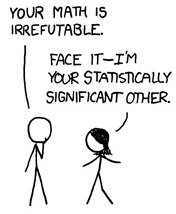
\includegraphics[width=.5\textwidth]{xkcd-boyfriend}}		
		\end{columns}
	}
	%
	%

	%
	%
	\section{Statistical hypotheses}
	%
	%

	%
	%
	\subsection{Statistical hypotheses}
	%
	%

	\begin{frame}[t]{Statistical hypotheses}
		
		\href{http://reason.org/}{From the Reason ``free minds and free markets'' Foundation}:\\[1em]

		\begin{quote}
		``A number of theorists assume that drinking has harmful economic effects, but data show that \textbf{drinking and earnings are positively correlated}. \textbf{\red{We hypothesize that drinking leads to higher earnings by increasing social capital.}} If drinkers have larger social networks, their earnings should increase. Examining the General Social Survey, we find that self-reported drinkers earn 10-14 percent more than abstainers, which replicates results from other data sets.''\\[1em]
		
		(\href{http://reason.org/news/show/127594.html}{B. L. Peters, E. Stringham, ``No Booze? You May Lose'', 2006.})
		\end{quote}

		\red{$H_1$:} ``An increase in social drinking leads to an increase in earnings.''
	\end{frame}
	%
	%

  \begin{frame}[plain, c]{}

		\begin{center}
			\href{http://www.phdcomics.com/comics.php?f=1563}{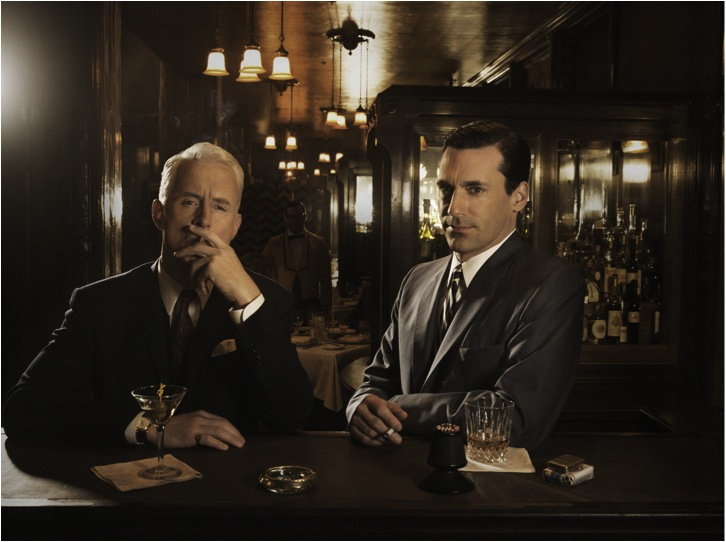
\includegraphics[width=\textwidth]{mad-men}}
    \end{center}
		  
  \end{frame}
	%
	%
	
	\begin{frame}[t]{Statistical hypotheses}
		
		\begin{block}{Substantive, directional hypotheses}
			$H_1: \red{\pm} \textsf{social drinking}~(\rightarrow \pm\textsf{social capital}) \rightarrow \red{\pm} \textsf{earnings}$\\
			$H_2: \red{\pm} \textsf{earnings}~(\rightarrow \pm\textsf{disposable income}) \rightarrow \red{\pm} \textsf{social drinking}$\\
		\end{block}

		\begin{block}{Rejecting the null hypothesis $H_0$}
			\red{$H_0$:} \red{no relationship} between social drinking and earnings\\
			\red{$H_a$:} \red{any relationship} between social drinking and earnings\\[.5em]
		\end{block}
		
		\begin{alertblock}{Proof by contradiction}
			
			\begin{enumerate}
				\item Get approximate upper bound of \textbf{\emph{p}-value} %
					$p \sim Pr(H_0)$
				\item Reject or retain $H_0$ at %
					\textbf{level of confidence} $\alpha \sim 0.05$ (or $0.01$)
			\end{enumerate}
			
		\end{alertblock}
		
	\end{frame}
	%
	%

	% \begin{frame}{Hypothesis testing}
	% 	 
	% 	\begin{block}{Substantive hypotheses}
	% 		$H_A$: There is an association between $X$ and $Y$, ...
	% 		
	% 		$H_\Delta$: There is a difference of $X$ between groups of $Y$, ...
	% 	\end{block}
	% 	
	% 	\begin{block}{Null hypothesis tests}
	% 		$H_0$: the association of $X$ and $Y$ is likely to be random.
	% 
	% 		$H_0$: the difference in $X$ between groups of $Y$ is likely to be random.
	% 	\end{block}
	% 	
	% 	\begin{alertblock}{Rejecting the null}
	% 		$H_0$ estimates the likelihood of an association or difference being attributable to \red{sampling error} under a certain \red{level of confidence}.
	% 	\end{alertblock}
	% 	
	% \end{frame}
	%
	%
	
	%
	%
	\section{Significance tests}
	%
	%

	\begin{frame}[t]{Significance tests}

		\begin{block}{Comparing differences}

			\begin{itemize}
				\item Comparing means: $H_0$: $\Delta = \bar{X} - \bar{Y} = 0$ %
					\hfill \code{ttest}
				\item Comparing proportions: $H_0$: $\Delta = Pr(X) - Pr(Y) = 0$ %
					\hfill \code{prtest}
			\end{itemize}
		\end{block}
		
		\begin{block}{Comparing distributions}

			\begin{itemize}
				\item $\chi^2$-test: observed vs. expected percentages %
					\hfill \code{tabchi}
				\item Odds ratios: success vs. failure rates %
					\hfill \code{tabodds}
			\end{itemize}

		\end{block}

	\end{frame}
	%
	%

	\begin{frame}[c]{$t$-test}

		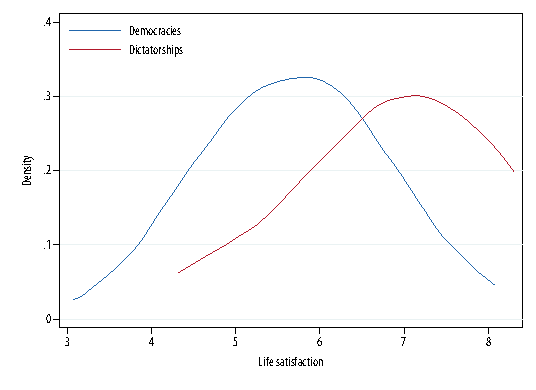
\includegraphics[width=\textwidth]{two-groups}

	\end{frame}
		
	\begin{frame}{$t$-test}
		
		\begin{block}{Measuring association as the difference in means between two groups of i.i.d.~observations:}
		
			\begin{itemize}
				\item Population notation:
				$\delta = \mu_1 - \mu_2$

				\item Sample notation:
				$D = \bar X_1 - \bar X_2$
			\end{itemize}

		\end{block}
		
		\begin{block}{The $t$-test computes a 95\% CI around the difference of their means and returns its $p$-value against the $t$-distribution.}
		
			\begin{itemize}
				\item Null hypothesis $H_0$:
				$\mu_1 - \mu_2 = 0$
			
				\item Test statistic:
				$t = \frac{D}{SE_D}$
			\end{itemize}

		\end{block}
		
	\end{frame}
	%
	%
	
	\begin{frame}[t]{$t$-test}
		
		\begin{block}{\texttt{ttest y, by(x)}}

			\begin{itemize}
				\item \texttt{y} is continuous, \texttt{x} is a dummy
				\item use \texttt{prtest} if \texttt{y} is also a dummy (proportions test)
				\item use \texttt{tab, gen()} to create dummies from categorical variables
			\end{itemize}

		\end{block}

        \begin{exampleblock}{Class exercise}
								
					\begin{itemize}
						\item \texttt{use data/qog2011, clear}
						\item \texttt{ttest gol\_enep, by(gol\_est2)}
						\item \texttt{prtest no\_mes, by(gol\_polreg)}
					\end{itemize}
			
        \end{exampleblock}
	
	\end{frame}
	%
	%
	
	% \begin{frame}[t]{$t$-test}
	% 
	% 	% \begin{block}{\texttt{prtest v1, by(v2)}}
	% 	% 
	% 	% 	\begin{itemize}
	% 	% 		\item \texttt{v1} and \texttt{v2} are both dummies (proportions) 
	% 	% 		\item the rest of the test works (almost) like the $t$-test
	% 	% 	\end{itemize}
	% 	% 
	% 	% \end{block}
	% 	
	% 	% \begin{exampleblock}{\texttt{use data/qog2011, clear}}
	% 	% 	
	% 	% 	% \begin{itemize}
	% 	% 	% 	\item Run a proportions test: \texttt{prtest no\_mes, by(gol\_polreg)}
	% 	% 	Explore the variables and interpret the output below.
	% 	% 	% \end{itemize}
	% 	% 				
	% 	%     \end{exampleblock}
	% 
	% 	\begin{center}
	% 		\includegraphics[width=.8\textwidth]{prtest-mes}
	% 	\end{center}
	%         
	% \end{frame}
	
	\begin{frame}[c]{Chi-squared test}

		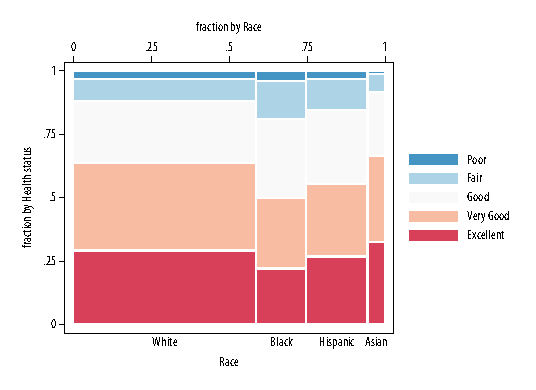
\includegraphics[width=\textwidth]{spineplot-health}
		
	\end{frame}
	%
	%

	% \begin{frame}[c]{\texttt{spineplot}}
	% 
	% 	\includegraphics[width=\textwidth]{spineplot-marstat}
	% 			
	% \end{frame}
	
	%
	%

	\begin{frame}{Chi-squared test}
		
		% Nonparametric test of association that measures the deviation in orthogonality between groups:
		
		\begin{block}{Definition}
		
			\begin{itemize}
				\item Null hypothesis $H_0$:
				$\chi^2=0$
			
				\item Test statistic:
				%
				$\chi^2=\sum_{i=1}^{n} \frac{(O_i - E_i)^2}{E_i}$ (deviation between observed frequencies $O_i$ and expected frequencies $E_i$ for each table cell $i$)
				
			\end{itemize}

		\end{block}
		
		\begin{block}{\texttt{tab y x, \red{exp chi2 V}}}

			\begin{itemize}
				\item add \texttt{V} to measure the association with Cramér's $V$ ($0 < V < 1$)
				\item use \texttt{tabchi} to inspect residuals, \texttt{tabodds} for odds ratios
			\end{itemize}

		\end{block}
		
	\end{frame}
	%
	%
	
	\begin{frame}[t]{Chi-squared test}
		
		\begin{exampleblock}{use data/nhis2009, clear}
		
			\begin{itemize}
				\item Variables: \texttt{d raceb marstat}
							
				\item Analyze the frequencies and residuals with \texttt{tabchi}
								
				\item \texttt{use data/qog2011, clear}
				\item \texttt{ttest gol\_enep, by(gol\_est2)}
				\item \texttt{prtest no\_mes, by(gol\_polreg)}
			
			\end{itemize}

		\end{exampleblock}
		
		\begin{center}
			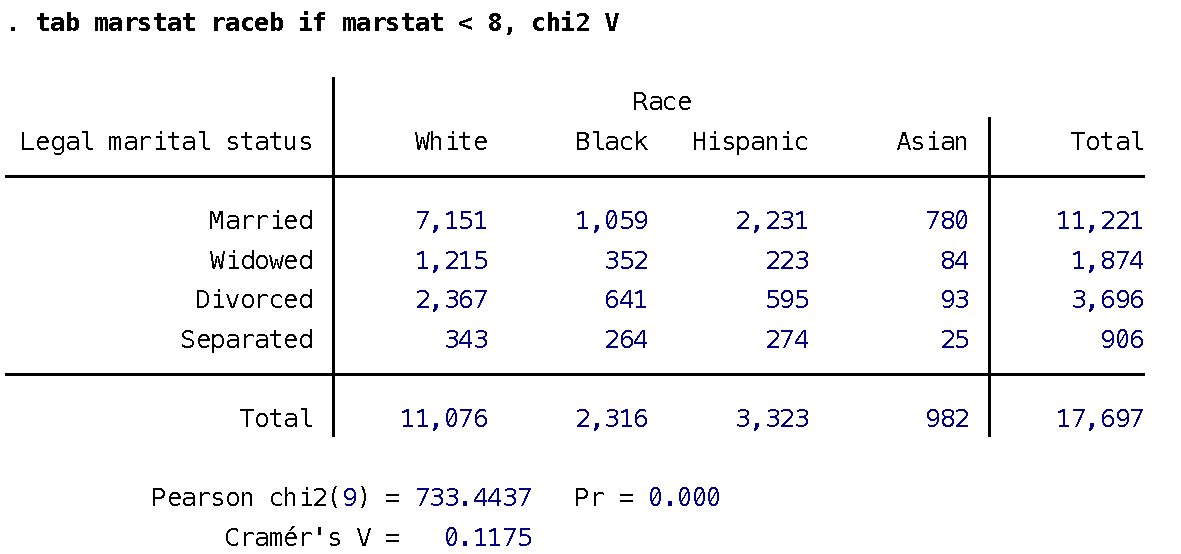
\includegraphics[width=.8\textwidth]{chi2-marstat}
		\end{center}
		
	\end{frame}
	%
	%
	
	%
	%
	\section{Type I and II Errors}
	%
	%

	\begin{frame}[t]{Type I and II Errors}

		\begin{block}{\textbf{Type I Error:} rejecting $H_0$ %
					when it is actually true}

			``Last year executed man proven innocent by DNA evidence.''
					
			\begin{itemize}
				\item $H_0$: presumption of innocence...
				\item $H_a$: ... until proven guilty (\red{$H_0$ wrongly rejected})
			\end{itemize}
		\end{block}
		
		\begin{block}{\textbf{Type II Error:} retaining $H_0$ %
					when it is actually false}

			``Violent father beats children after being released from custody.''
					
			\begin{itemize}
				\item $H_0$: parents considered responsible
				\item $H_a$: ... until proven abusive (\red{$H_0$ wrongly retained})
			\end{itemize}

		\end{block}

	\end{frame}
	%
	%

	\begin{frame}[c]{Type I and II Errors}
		
		\begin{columns}[c]
			\column{.5\textwidth}
			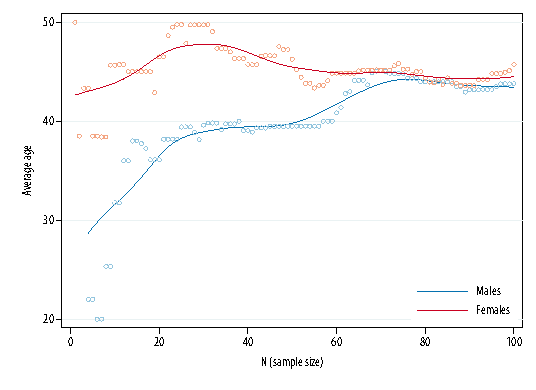
\includegraphics[width=\textwidth]{diff-age}
			
			\begin{center}
				Type I error
			\end{center}

			\column{.5\textwidth}
			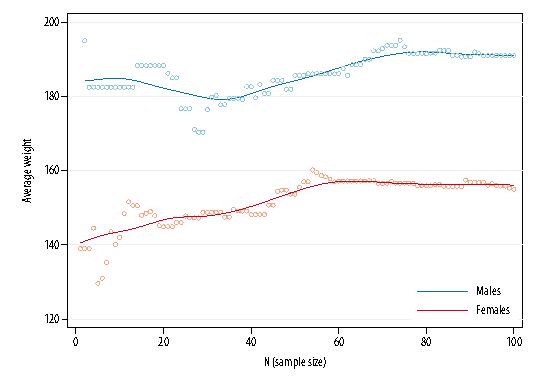
\includegraphics[width=\textwidth]{diff-weight}

			\begin{center}
				Type II error
			\end{center}
		\end{columns}
		
	\end{frame}
	%
	%
	
  \begin{frame}[plain, c]{Estimation is powerful}

		\begin{center}
			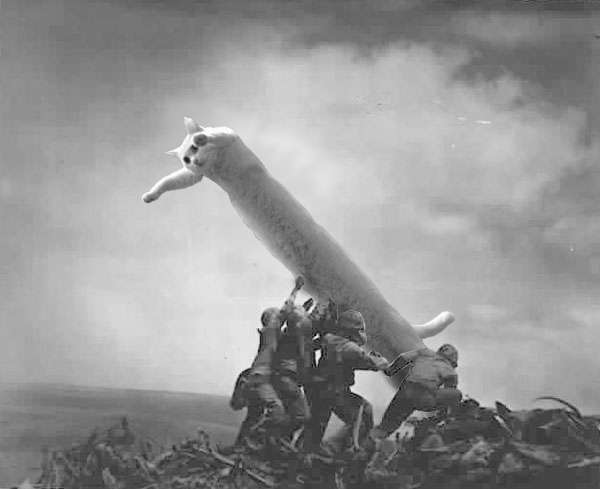
\includegraphics[height=.7\textheight]{longcat-prophecy-white}
    \end{center}
		  
  \end{frame}
	%
	%
	
  \begin{frame}[plain, c]{Significance is deceptive}

		\begin{center}
			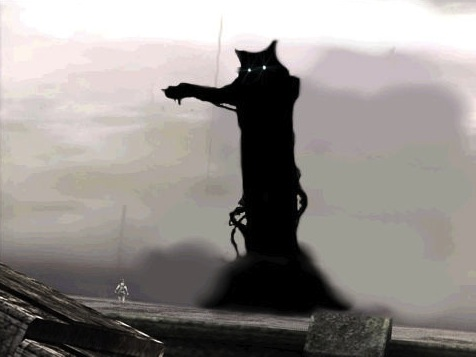
\includegraphics[height=.7\textheight]{longcat-prophecy-black}
    \end{center}
		  
  \end{frame}
	%
	%
	
  \begin{frame}[plain, c]{}

		\begin{center}
			
\includegraphics[width=\textwidth]{longcat-prophecy}
    \end{center}
		  
  \end{frame}
	%
	%
	
% 	
% 	\subsection*{The Prophecy}
% 
% % img-longcat-tao.jpg
% 
% 	% The efforts to raise the powers of Estimation Cat are considerable...
% 	\fullslide{images/longcat-prophecy1.jpg}
% 
% 	\begin{frame}[t]{The Prophecy}
% 
% 	The Prophecy requires \textbf{raising the power of \red{Estimation Cat}}\\as much as possible:
% 	
% 	\begin{columns}[T]
% 		\column{.625\textwidth}
% 		\begin{itemize}
%  			\item \textbf{Maximise sample size:} missing observations and/or low $n$ reduce the \red{statistical power} of your sample.
% 
%  			\item \textbf{Approach normality:} Estimation Cat is pleased when your variables follow a \red{normal distribution}.
% 
%  			\item \textbf{Use the appropriate test:} significance tests come with \red{restrictive assumptions}, e.g. independent groups, equal variance.
% 		\end{itemize}
% 
% 	This is difficult: Estimation Cat is needy.	
% 
% 		\column{.3\textwidth}
% 	\vspace{0em}
% 	\begin{flushright}
% 	\includegraphics[scale=.3]{images/longcat.jpg}		
% 	\end{flushright}
% 	\end{columns}
% 		
% 	\end{frame}
% 
% 	% ... But the threat of Significance Cat looms over the mere mortal researcher.
% 	\fullslide{images/longcat-prophecy2.jpg}
% 
% 	\begin{frame}[t]{The Prophecy}
% 
% 	The Prophecy also requires \textbf{curbing the threat of \red{Significance Cat}} as much as possible:
% 	
% 	\begin{columns}[T]
% 		\column{.625\textwidth}
% 		\begin{itemize}
%  			\item \textbf{Maximise sample size} (again): the number of observations restricts the \red{degrees of freedom} used to calculate $p$-values from \red{Student's $t$-distribution}.
% 
%  			\item \textbf{Use the appropriate test} (again): a correct reading of an inappropriate test is a \red{Type III Error} (providing the right answer to the wrong question).
% 		\end{itemize}
% 
% 	This is also difficult, especially given the cunning nature of Significance Cat.	
% 
% 		\column{.3\textwidth}
% 	\vspace{0em}
% 	\begin{flushright}
% 	
\includegraphics[scale=.3]{images/longcat-black.jpg}		
% 	\end{flushright}
% 		
% 	\end{columns}
% 	\end{frame}
% 	
% 	\begin{frame}[t]{The Prophecy}
% 
% 	The Prophecy is chiefly achieved through \textbf{statistical reasoning} that carefully balances the awesome powers of \red{estimation} and \red{significance}:
% 	
% 	\begin{columns}[T]
% 		\column{.625\textwidth}
% 		\begin{itemize}
%  			\item \textbf{Keep an open mind}: reading $p$-values require paying attention to \red{Type I and Type II Errors}. The key to any test remains interpretation.
% 
%  			\item \textbf{Avoid cargo cults:} statistical inference is a probabilistic method. Each test result is expressed as a \red{likelihood} that carries no absolute certainty.
% 		\end{itemize}
% 		\column{.3\textwidth}
% 	\vspace{0em}
% 	\begin{flushright}
% 	
\includegraphics[width=\textwidth]{images/longcat-tao.jpg}		
% 	\end{flushright}		
% 	\end{columns}
% 	
% 		\vspace{1em}
% 		And yes, this amounts to a lot of computational and intellectual effort for the incomplete and imperfect results of frequentist statistics.	
% 		
% 	\end{frame}

	%
	%
	\section{Practice}
	%	
	%
  
	\begin{frame}[t]{Practice session}

    \begin{block}{Class}
      \comm{Get the do-file for this week.}\\
      \code{srqm\_get week6.do}\\
      
			\comm{Open to read and replicate.}\\
			\code{doedit code/week6}\\    
    \end{block}

    \begin{alertblock}{Coursework}
      \begin{itemize}
	       \item Finish the do-file and read all comments at home.
	       \item Catch up on all readings %
				 	(see \href{http://f.briatte.org/teaching/quanti/}%
				 	{course website}).
	       \item Revise your code and paper after getting feedback.
      \end{itemize}
    \end{alertblock}
    		
	\end{frame}
  %
  %
	
\end{document}

